\chapter{Valutazione e conclusioni}\label{ch:valutazione}

Far passare i pacchetti attraverso una VM ha un costo in latenza e in throughput, che viene misurato con i test descritti nella sezione~\ref{sec:metodologia} e i cui risultati sono riportati nelle sezioni~\ref{sec:latenza} e~\ref{sec:throughput}. La sezione~\ref{sec:limiti} riassume poi i limiti di vnic, e la sezione~\ref{sec:conclusioni} chiude la tesi riprendendo gli obiettivi e proponendo alcuni sviluppi futuri.

\section{Ambiente e metodologia}\label{sec:metodologia}

I test confrontano vnic con una veth pair che collega direttamente \texttt{ns0} e \texttt{ns1}, senza VM. Le configurazioni sono quattro, riassunte nella tabella~\ref{tab:configurazioni}. Quella senza programma isola il costo della sola VM, mentre le ultime due valutano vnic come viene usato normalmente, cioè con un filtro caricato nelle due versioni disponibili.

\begin{table}[H]
    \centering
    \begin{tabular}{@{}l >{\raggedright\arraybackslash}p{0.6\linewidth}@{}}
    \toprule
    \textbf{Configurazione} & \textbf{Descrizione} \\
    \midrule
    veth & \texttt{ns0} e \texttt{ns1} collegati da una sola veth pair, senza VM \\
    no prog. & vnic senza programma, la VM inoltra tutti i frame \\
    eBPF & vnic con il filtro \texttt{drop-udp} in eBPF \\
    P4 & vnic con il filtro \texttt{drop-udp} in P4 \\
        \bottomrule
\end{tabular}
    \caption{Configurazioni usate nei test}
    \label{tab:configurazioni}
\end{table}

Il filtro \texttt{drop-udp} scarta solo i pacchetti UDP, mentre i test usano traffico ICMP e TCP. In tutte le configurazioni, quindi, i pacchetti arrivano a \texttt{ns1}, così da valutare quanto vnic incida sul traffico ammesso.  

La latenza è misurata come round trip time (RTT) con \texttt{ping} da \texttt{ns0} a \texttt{ns1}. Vengono inviate 1000 richieste, una ogni 5\,ms, e alla fine \texttt{ping} riporta il RTT medio e la sua deviazione standard (\texttt{mdev}). Prima del test vengono inviati 20 ping, che non sono considerati, così che per esempio la risoluzione dell'indirizzo MAC con ARP non influisca sui risultati.

Il throughput è misurato inviando con \texttt{socat} un file da 1\,GiB di dati casuali da \texttt{ns0} a \texttt{ns1} su una connessione TCP. Il file si trova in memoria (\texttt{/dev/shm}) e il ricevente scrive i dati in \texttt{/dev/null}, per cui il disco non interviene e non influisce sul risultato. Il tempo va dall'avvio del mittente alla chiusura del ricevente, e il throughput è la dimensione del file divisa per questo tempo. Per ogni configurazione il file viene inviato 5 volte.

Ogni test è ripetuto in tre round, e in ogni round vnic viene avviato da capo per ciascuna configurazione. Si hanno quindi tre valori di RTT medio e 15 trasferimenti totali per configurazione. L'intero benchmark è eseguito in automatico dallo script \texttt{scripts/bench.sh}.

I test sono stati eseguiti su un portatile con processore AMD Ryzen AI 7 350 (8 core e 16 thread) e 16\,GB di RAM, con openSUSE Tumbleweed (kernel 7.2.7), QEMU 11.1.1 con KVM e clang 23.1.1. Per la versione in P4, \texttt{p4c-ebpf} è stato eseguito nel container.
La VM è quella descritta nel capitolo~\ref{ch:implementazione}, cioè Debian 12 con kernel 6.1, 2 CPU virtuali, 1\,GB di RAM e interfacce virtio-net con una sola coda. Il portatile era collegato all'alimentatore, con il profilo energetico \texttt{performance}.

\section{Latenza}\label{sec:latenza}

La tabella~\ref{tab:latenza} riporta il RTT medio rilevato da \texttt{ping} in ciascun round.

\begin{table}[H]
    \centering
    \begin{tabular}{@{}lrrr@{}}
        \toprule
        \textbf{Configurazione} & \textbf{Round 1} & \textbf{Round 2} & \textbf{Round 3} \\
        \midrule
        veth & $<1$ & $<1$ & $<1$ \\
        no prog. & 207 & 196 & 175 \\
        eBPF & 204 & 184 & 141 \\
        P4 & 146 & 172 & 194 \\
        \bottomrule
    \end{tabular}
    \caption{RTT medio da \texttt{ns0} a \texttt{ns1} in $\mu$s (1000 ping per round)}
    \label{tab:latenza}
\end{table}

Senza VM il RTT medio è inferiore a 1\,$\mu$s, al limite della risoluzione di \texttt{ping}, mentre con la VM è tra 0,14 e 0,21\,ms, cioè di circa due ordini di grandezza più alto. Infatti ogni ping attraversa la VM due volte, all'andata e al ritorno, e ogni volta passa da QEMU e dal bridge \texttt{brVM}. Il programma XDP, però, viene eseguito solo all'andata.

Tra le tre configurazioni con la VM, invece, non c'è una differenza sistematica. I valori di una stessa configurazione cambiano da un round all'altro anche di 60\,$\mu$s (con il filtro in eBPF vanno da 141 a 204\,$\mu$s), cioè più della differenza tra le medie delle configurazioni, e la configurazione più veloce nel primo round, P4, è la più lenta nel terzo. Anche all'interno di un round la deviazione standard è tra 23 e 54\,$\mu$s. Un filtro che controlla pochi campi degli header richiede un tempo trascurabile rispetto all'attraversamento della VM, per cui la variabilità dipende probabilmente dalla VM stessa. Con un ping ogni 5\,ms la VM resta quasi sempre inattiva, quindi a ogni pacchetto le sue CPU virtuali devono essere risvegliate, con tempi che cambiano da un pacchetto all'altro e da un avvio all'altro.

vnic aggiunge quindi circa 0,15--0,2\,ms al RTT, mentre il costo del programma XDP è troppo piccolo per essere rilevato in questo modo.

\section{Throughput}\label{sec:throughput}

La figura~\ref{fig:bench-throughput} riporta, per ciascuna configurazione, il throughput medio dei 15 trasferimenti.

\begin{figure}[H]
    \centering
    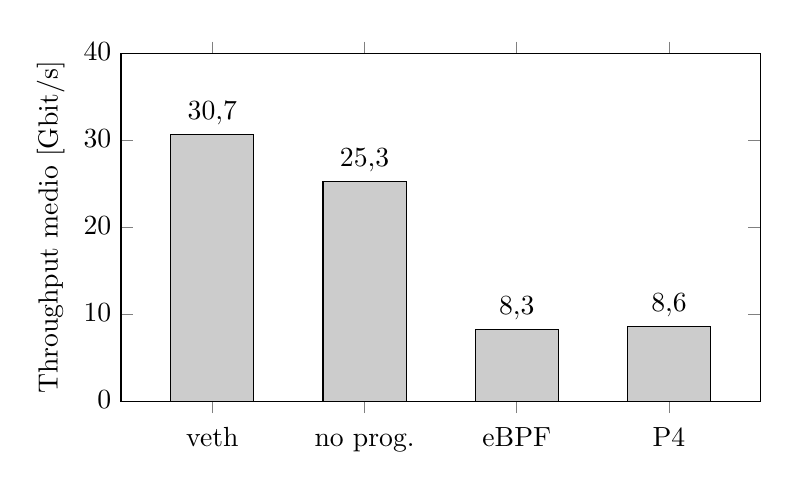
\begin{tikzpicture}
\begin{axis}[
    ybar,
    width=0.8\textwidth, height=6cm,
    symbolic x coords={veth, noprog, ebpf, p4},
    xtick=data,
    typeset ticklabels with strut,
    xticklabels={veth, no prog., eBPF, P4},
    ylabel={Throughput medio [Gbit/s]},
    ymin=0, ymax=40,
    bar width=30pt,
    enlarge x limits=0.2,
    nodes near coords,
    nodes near coords style={/pgf/number format/.cd, fixed, precision=1, use comma},
]
\addplot[fill=gray!40, draw=black] coordinates {(veth,30.7) (noprog,25.3) (ebpf,8.3) (p4,8.6)};
\end{axis}
\end{tikzpicture}

    \caption{Throughput medio nell'invio di un file da 1\,GiB da \texttt{ns0} a \texttt{ns1} (15 trasferimenti per configurazione)}
    \label{fig:bench-throughput}
\end{figure}

Con la veth diretta il throughput medio è di 30,7\,Gbit/s, con valori molto stabili, da 28,8 a 32,2\,Gbit/s. Con la VM senza programma XDP scende in media a 25,3\,Gbit/s, ma è molto più variabile, con 11 trasferimenti su 15 tra 19,7 e 21,7\,Gbit/s e gli altri 4 sopra i 35\,Gbit/s. Attraversare la VM ha quindi un costo, ma il throughput resta dello stesso ordine di grandezza di quello della veth diretta. Valori così alti sono possibili grazie agli offload di segmentazione, per cui i dati TCP attraversano le interfacce virtuali in pacchetti aggregati fino a 64\,KB, invece che in frame da 1500 byte come su una rete reale.

Con il filtro caricato, invece, il throughput scende a circa 8,5\,Gbit/s (8,3 in eBPF e 8,6 in P4), cioè circa tre volte meno che senza programma. Come visto nella sezione~\ref{sec:punti-comuni}, quando si carica un programma XDP il driver \texttt{virtio\_net} della VM disattiva gli offload di ricezione~\cite{virtio-net-src}. Da quel momento QEMU non può più consegnare alla VM pacchetti aggregati, ma solo frame da al massimo 1500 byte, ognuno dei quali viene passato alla VM ed elaborato dal programma singolarmente. A parità di dati trasferiti, quindi, i pacchetti da gestire sono molti di più.

Le due versioni del filtro hanno lo stesso throughput. La differenza tra le due medie, 0,3\,Gbit/s, è più piccola di quella tra i round di una stessa configurazione. Con il filtro in eBPF, per esempio, la media di un round va da 7,5 a 8,8\,Gbit/s.

\section{Limiti}\label{sec:limiti}

Riassumendo quanto emerso nei capitoli precedenti, vnic ha i seguenti limiti:
\begin{itemize}
    \item ogni interfaccia della VM ha una sola coda di ricezione, per cui non c'è distribuzione dei pacchetti tra più code e \texttt{rx\_queue\_index} vale sempre 0;
    \item il programma elabora solo il traffico da \texttt{ns0} verso \texttt{ns1}, mentre quello di ritorno attraversa la VM senza passare da alcun programma;
    \item un REDIRECT verso \texttt{ens4} funziona solo se anche \texttt{ens4} ha un programma XDP, che vnic non carica;
    \item manca un piano di controllo, per cui dall'host non si possono leggere né modificare le mappe e le tabelle del programma. Senza contatori, dall'esterno della VM DROP e ABORTED sono indistinguibili;
    \item se il verifier rifiuta il programma, \texttt{up} termina comunque senza errori e il motivo del rifiuto compare solo nel log della VM;
    \item i programmi P4 sono limitati al modello \texttt{ebpfFilter}, che permette solo di accettare o scartare i pacchetti;
    \item le prestazioni ottenute con vnic non rappresentano quelle di una SmartNIC, perché il programma viene eseguito dalla CPU dell'host attraverso una VM, e il suo caricamento disattiva anche gli offload della scheda virtuale;
    \item l'avvio richiede circa 30 secondi in tutte le configurazioni, quasi tutti dovuti al boot della VM. Con P4, se il compilatore viene eseguito nel container, si aggiungono alcuni secondi per la traduzione;
    \item \texttt{up} e \texttt{down} richiedono i privilegi di root, e può essere attiva una sola istanza alla volta.
\end{itemize}

\section{Conclusioni e sviluppi futuri}\label{sec:conclusioni}

Concludiamo riprendendo gli obiettivi elencati nella sezione~\ref{sec:obiettivi} e confrontandoli con i risultati ottenuti nei capitoli precedenti.

Il primo era eseguire programmi eBPF e P4 come su una SmartNIC. vnic emula la scheda con una macchina virtuale posta tra due network namespace e vi carica il programma dell'utente, che elabora i pacchetti in arrivo prima che raggiungano il resto del sistema, come farebbe sulla scheda reale. I programmi P4 vengono prima tradotti in eBPF e, con il modello \texttt{ebpfFilter}, possono solo accettare o scartare i pacchetti.

Il secondo era verificarne il comportamento con traffico di rete controllato. Con vnic l'utente può inviare i pacchetti che preferisce e osservare quali attraversano la scheda emulata e quali vengono scartati, come mostrato nel capitolo~\ref{ch:casouso}. Gli esempi della repository eseguono questa verifica in automatico, sia in eBPF sia in P4.

Il terzo era capire che cosa l'emulazione rappresenta fedelmente e quanto costa. La logica del programma viene eseguita come su una SmartNIC reale, mentre alcuni aspetti della scheda, come le code di ricezione e gli offload hardware, non sono riprodotti. Le misure mostrano che vnic aggiunge circa 0,2\,ms di latenza e che, con un programma caricato, il throughput scende a circa un terzo. vnic è quindi adatto a verificare la logica di un programma, ma non a valutarne le prestazioni.

Dai limiti elencati nella sezione~\ref{sec:limiti} derivano alcuni possibili sviluppi futuri:
\begin{itemize}
    \item sostituire l'immagine Debian e cloud-init con un kernel minimale e un piccolo filesystem per ridurre i tempi di boot;
    \item permettere di leggere e modificare dall'host lo stato del programma, per esempio dei contatori;
    \item emulare più code di ricezione, configurandole nelle interfacce virtio-net;
    \item elaborare anche il traffico di ritorno e permettere il REDIRECT tra le due interfacce della VM;
    \item permettere di avviare più istanze contemporaneamente.
\end{itemize}